%!TEX TS-program = xelatex
%!TEX options = -aux-directory=Debug -shell-escape -file-line-error -interaction=nonstopmode -halt-on-error -synctex=1 "%DOC%"
\documentclass{article}
\input{LaTeX-Submodule/template.tex}

% Additional packages & macros
\DeclareMathOperator*{\argmin}{arg\,min}

% Header and footer
\newcommand{\unitName}{Machine Learning}
\newcommand{\unitTime}{Semester 1, 2024}
\newcommand{\unitCoordinator}{Dr Simon Denman}
\newcommand{\documentAuthors}{Tarang Janawalkar}

\fancyhead[L]{\unitName}
\fancyhead[R]{\leftmark}
\fancyfoot[C]{\thepage}

% Copyright
\usepackage[
    type={CC},
    modifier={by-nc-sa},
    version={4.0},
    imagewidth={5em},
    hyphenation={raggedright}
]{doclicense}

\date{}

\begin{document}
%
\begin{titlepage}
    \vspace*{\fill}
    \begin{center}
        \LARGE{\textbf{\unitName}} \\[0.1in]
        \normalsize{\unitTime} \\[0.2in]
        \normalsize\textit{\unitCoordinator} \\[0.2in]
        \documentAuthors
    \end{center}
    \vspace*{\fill}
    \doclicenseThis
    \thispagestyle{empty}
\end{titlepage}
\newpage
%
\tableofcontents
\newpage
%
\section{Introduction}
Machine learning is a field of computer science concerned with the
development of statistical algorithms that enable computer systems to
learn insights from data. Machine learning is a multi-disciplinary
field that is related to statistics, pattern recognition, data mining,
and artificial intelligence.
\subsection{Machine Learning Process}
Broadly speaking, there are three steps to enable machines to learn.
\begin{enumerate}
    \item \textbf{Input Data}: A model must be provided with input data.
          This data consists of audio, images, text, or any other form
          of data, which enables us to build a model. Ideally, it
          is desirable to have a large amount of data, as this produces
          a more accurate model, and removes the possibility of
          overfitting when many features are present.
    \item \textbf{Data Abstraction}: To effectively train a model on
          this data, it needs to be abstracted into a consistent format
          that can be understood by a model. This includes
          pre-processing the data, removing any noise or irrelevant
          features, and ensuring that the dimensionality (or the number
          of features) is the same across all samples.
    \item \textbf{Generalisation}: When data is ready, we can use a
          machine learning technique to determine whether a model
          generalises well to new data.
\end{enumerate}
\subsection{Machine Learning Paradigms}
There are three main types of machine learning paradigms:
\begin{itemize}
    \item \textbf{Supervised Learning}: In this type of learning, a
          model is provided both input and expected output data. The
          purpose here is to learn a mapping from input to output, to
          predict an output for new unseen data.

          For example, we might provide a model a video of pedestrians
          with a person count in each frame. The model then regresses
          features such as size, texture, and shape to predict the
          number of people in unseen frames.

          Another related example may include object tracking, where a
          model learns to track objects in a video, given a
          pre-labelled set of frames with tracked objects.
    \item \textbf{Unsupervised Learning}: In this type of learning, a
          model is provided only input data, and is mainly used for
          knowledge discovery---to find order and characteristics in
          data.

          An example of this is clustering, where a model might group
          people who are walking together, based on their motion
          characteristics.

          Another example is the detection of anomalies or abnormal
          behaviour in data. For example, a model may be trained on
          pedestrian motion, and use unsupervised learning to track
          vehicles and bicycles in a pedestrian zone.
    \item \textbf{Reinforcement Learning}: In this type of learning, a
          model learns to make decisions by interacting and responding
          to an environment. The model is rewarded or penalised based on
          its actions, and its goal is to learn the best sequence of
          actions to maximise its reward.

          An example of this may be a robot learning to walk. The
          objective might be to maximise the distance travelled in one
          direction.
\end{itemize}
\subsection{Importance of Data}
Data is the most important aspect of machine learning, both in terms of
\textbf{quality and quantity}. A high-quality dataset that is well
prepared and which covers all possible cases considered in a model,
leads to better outcomes.
\begin{itemize}
    \item a model cannot produce predictions that are better than the
          data it is trained on
    \item a model cannot compensate for errors in the annotation of
          data
\end{itemize}
It is also important to consider \textbf{data diversity} to ensure that
a model does not learn \textbf{biases} present in the data. For example,
a male dominated dataset may lead to a model that is biased against
women.

Data also suffers from the \textit{curse of dimensionality}. Datasets
often have:
\begin{itemize}
    \item a large number of dimensions or features (i.e., columns,
          observed variables)
    \item but a small number of samples (i.e., rows, observations)
\end{itemize}
In such cases, the feature space is sparsely populated and the model
may \textbf{overfit}. Every new feature increases the complexity
of the model, and also necessitates more data, to produce an accurate
model---this number depends on the type of classifier or learning
algorithm used, and therefore a model should be kept simple.
\subsection{Data Splitting}
To efficiently train and evaluate a model, we can split the data into
three sets:
\begin{itemize}
    \item \textbf{Training Set}: This set is used to train the model.
    \item \textbf{Validation Set}: This set is used to tune model
          hyperparameters to evaluate a model's performance. The training
          set will be trained using different hyperparameters to evaluate
          which set of hyperparameters produce the best model.
    \item \textbf{Test Set}: This set is used to evaluate the model's
          performance on unseen data.
\end{itemize}
This approach uses \textit{holdout validation} where data is
\textit{held out} for validation and/or testing, so that the training,
validation, and testing stages are completely separate. Note that this
requires datasets to be large enough to ensure that a model has enough
data for training.

When \textbf{insufficient data} is available, \textit{cross-validation}
can be used to dynamically split the dataset into training and
validation sets (i.e., a 80\% training/20\% validation split). This may
be repeated 5 times, so that each split is used as a validation set.
The best model is then selected based on the average performance across
all splits.

In some cases, machine learning \underline{may not be possible} if the
dataset is too small. This may be because the data does not contain the
patterns and relationships that we are trying to learn. For some
problems, this threshold may be a few hundred samples, while for
others, it may be a few million. Extrapolation beyond the data may also
be problematic in such cases.
\subsection{Traditional Machine Learning to Deep Learning}
\subsubsection{Traditional Machine Learning}
The traditional machine learning pipeline typically consists of:
\begin{itemize}
    \item \textbf{Pre-processing}: Preparing data for a model using
          normalisation, scaling, noise reduction, etc.
    \item \textbf{Feature Extraction}: Extracting features from data;
          MFCC (audio), HOG (image/video), and bag-of-words (text).

          This step is often informed by the task. For example, if we
          need to recognise shapes in images, we might use a technique
          that captures edge detection. In the case of audio, we might
          use a technique that captures frequency information.
    \item \textbf{Machine Learning}: Passing the features to a model
          using a machine learning technique.
\end{itemize}
In this model, features are \textbf{hand-crafted}, and based on domain-specific
knowledge. Choosing the optimal features for a given problem can be a
tedious and iterative process. This leads to different formulations for
different tasks, and may significantly increase the complexity of a
problem, especially when we need to extract multiple sets of features.
\subsubsection{An Aside on Neural Networks}
A neural network is modelled after the human brain and nervous system.
It is built on a single unit or \textbf{node} called a \textit{neuron},
in which data is passed through a series of \textbf{layers}, each of
which is connected to other neurons through \textbf{edges}. Neural
networks typically consist of a large number of parameters and many
interconnections.

Choosing the appropriate number of layers in a neural network (or the
\textit{depth} of a neural network), is problem dependent. A higher
depth allows us to learn \textit{higher level features}, and contains
more parameters, but this is often harder to learn and also increases
the likelihood of overfitting. Larger networks also require more data,
and therefore more memory and computational resources.
\subsubsection{Deep Learning}
Deep learning is a subset of machine learning that uses neural networks
to learn features from data. It differs from the traditional machine
learning pipeline in that it does not require manual feature
extraction, but instead learns it's own representation from
pre-processed data. This makes deep learning more \textbf{adaptable} to
different tasks, and also reduces the complexity of a problem.

A downside of deep learning is that models are often extremely large
compared to traditional approaches;
\begin{itemize}
    \item a traditional machine learning model may have a few hundred
          parameters
    \item a deep learning model may have millions of parameters
\end{itemize}
This leads to an increase in computational resources required to train
and evaluate a model, and also makes a model difficult to interpret.

In deep learning, feature engineering is replaced with \textbf{network
engineering}, where we must carefully choose the appropriate
architecture for a problem. This includes:
\begin{itemize}
    \item the number of layers,
    \item the number of neurons in each layer, and
    \item the type of activation function used.
\end{itemize}
This is often an iterative process, and it may not be feasible to find
the optimal architecture for a given problem, through exhaustive
testing.
\section{Linear Regression}
A simple model for predicting the relationship between a dependent
variable \(y\) (\textbf{response}), and an independent variable \(x\)
(\textbf{predictor}), is a straight line. Given a set of \(n\)
input-output pairs \(\left( x^{\left( i \right)},\: y^{\left( i
\right)} \right)\), we can model a linear relationship between \(x\)
and \(y\) as:
\begin{equation*}
    y^{\left( i \right)} = \beta_0 + \beta_1 x^{\left( i \right)}
\end{equation*}
where \(\beta_0\) is the \(y\)-\textbf{intercept} and \(\beta_1\) is the
\textbf{gradient} of the line. In practice, data rarely fits a model
perfectly and therefore, we will assume the relationship:
\begin{equation*}
    \hat{y}\left( x \right) = \hat{\beta}_0 + \hat{\beta}_1 x
\end{equation*}
where \(\hat{y}\) is known as the \textbf{hypothesis function} which
\textbf{predicts} value of \(y\), and \(\hat{\beta}_0\) and
\(\hat{\beta}_1\) are the \textbf{estimated} values of the
\textbf{parameters} \(\beta_0\) and \(\beta_1\), respectively. This
model adds a \textbf{residual} term \(\epsilon\) to account for the
error in each observation:
\begin{align*}
    y^{\left( i \right)} & = \hat{y}\left( x^{\left( i \right)} \right) + \epsilon^{\left( i \right)}         \\
                         & = \hat{\beta}_0 + \hat{\beta}_1 x^{\left( i \right)} + \epsilon^{\left( i \right)}
\end{align*}
here \(\epsilon\) is assumed to be normally distributed with zero mean
and \(\sigma^2\) variance:
\begin{equation*}
    \epsilon \overset{\mathrm{iid}}{\sim} \mathrm{N}\left( 0,\: \sigma^2 \right).
\end{equation*}
As \(y\) depends on \(\epsilon\), we can also show that
\begin{equation*}
    y \sim \mathrm{N}\left( \beta_0 + \beta_1 x,\: \sigma^2 \right)
\end{equation*}
where \(y\) is normally distributed for fixed values of \(x\).
The values of \(\hat{\beta}_0\) and \(\hat{\beta}_1\) arise when we
consider the \textbf{loss function}:
\begin{equation*}
    L\left( \symbf{\beta} \right) = \frac{1}{2} \epsilon^2 = \frac{1}{2} {\left( y - \hat{y} \right)}^2 = \frac{1}{2} {\left( y - \left( \beta_0 + \beta_1 x \right) \right)}^2.
\end{equation*}
which we wish to minimise. As these estimators apply to the entire
training set, we will consider the \textbf{cost function}:
\begin{equation*}
    J\left( \symbf{\beta} \right) = \frac{1}{n} \sum_{i = 1}^n L\left( \beta \right).
\end{equation*}
which averages the loss across all observations. The goal of this cost
function is to find the best parameters \(\hat{\symbf{\beta}}\) that minimise
the loss across all observations:
\begin{equation*}
    \hat{\symbf{\beta}} = \argmin_{\symbf{\beta}} J\left( \symbf{\beta} \right).
\end{equation*}
In this model, we must ensure that there are at least as many
observations as there are parameters to estimate.
\subsection{Correlation}
Correlation is a statistical relationship between two variables. This
measure allows us to determine the strength of a linear relationship
between two variables. One common measure of correlation is the
\textbf{Pearson correlation coefficient}, which is given by:
\begin{equation*}
    \rho_{xy} = \frac{\sigma_{xy}}{\sigma_x \sigma_y}
\end{equation*}
where \(\sigma_{xy}\) is the \textbf{covariance} between \(x\) and \(y\),
and \(\sigma_x\) and \(\sigma_y\) are the variances of \(x\) and \(y\),
respectively. Using the sample covariance\footnote{See
    \hyperref[appendix:numerical-summaries]{Appendix~\ref*{appendix:numerical-summaries}}
    for more details.}:
\begin{equation*}
    r_{xy} = \frac{s_{xy}}{s_x s_y}.
\end{equation*}
The sample covariance \(s_{xy}\) has the following characteristics:
\begin{itemize}
    \item \(s_{xy} > 0\): \(y\) increases as \(x\) increases
    \item \(s_{xy} < 0\): \(y\) decreases as \(x\) increases
    \item \(s_{xy} \approx 0\): no linear relationship between \(x\) and \(y\)
\end{itemize}
To generalise this measure across datasets, we often consider the
\textit{normalised} correlation coefficient \(r_{xy}\), which tells use
the strength of a linear relationship between two variables. The
following diagram shows various datasets and their correlation
coefficients:
\begin{figure}[H]
    \centering
    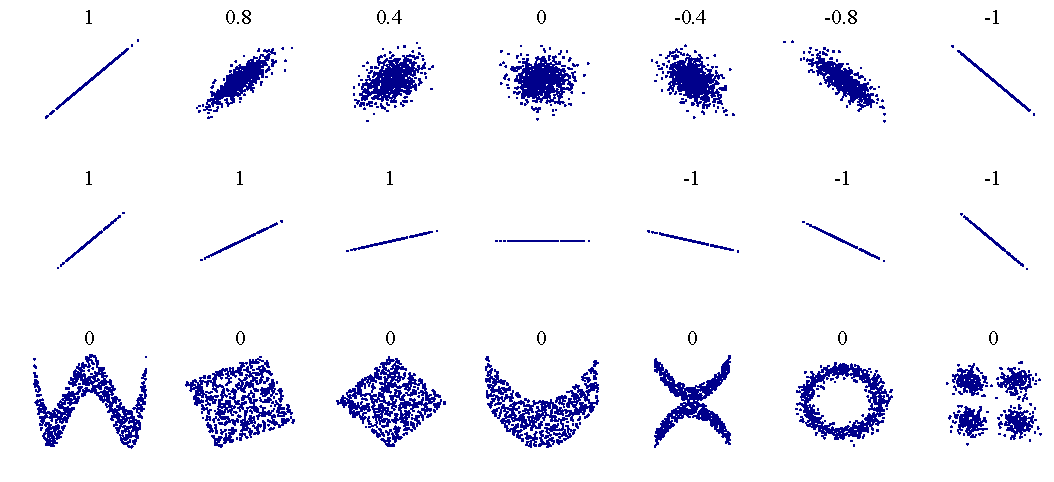
\includegraphics[width = \linewidth]{figures/correlation.pdf}
    \caption{Pearson correlation coefficient of \(x\) and \(y\) for several sets of points.} % \label{}
\end{figure}
There are a number of important points to note about the correlation
coefficient:
\begin{itemize}
    \item The correlation coefficient does not contain any information
          about the gradient, as is seen in the second row.
    \item A correlation coefficient of 0 indicates \textit{no linear
          relationship}, it does not imply that there is \textit{no
          relationship}, as is seen in the third row.
    \item The correlation coefficient does not imply
          \textit{causation}. Care must be taken when assuming that a
          relationship between two variables is causal.
\end{itemize}
To minimise redundancy in a model, it is crucial for predictors to be
correlated with response variables, and uncorrelated to other predictors.
\subsection{Simple Linear Regression}
Simple linear regression is a special case of linear regression, where
we have only one input variable \(x_1\), and we can use the method of
maximum likelihood estimation to estimate the parameters \(\beta_0\)
and \(\beta_1\):
\begin{align*}
    \hat{\beta}_1 & = \frac{\sum_{i = 1}^n \left( x^{\left( i \right)} - \bar{x} \right) \left( y^{\left( i \right)} - \bar{y} \right)}{\sum_{i = 1}^n {\left( x^{\left( i \right)} - \bar{x} \right)}^2} \\
    \hat{\beta}_0 & = \bar{y} - \hat{\beta}_1 \bar{x}
\end{align*}
where \(\bar{x}\) and \(\bar{y}\) are the sample means of \(x\) and \(y\),
respectively.
\subsection{Multiple Linear Regression}
In multiple linear regression, we consider a \(p\)-dimensional feature
space, or \(p\) input variables, with \(p + 1\) parameters to estimate.
Here hypothesis function generalises to:
\begin{equation*}
    \hat{y}\left( x \right) = \hat{\beta}_0 x_0 + \hat{\beta}_1 x_1 + \hat{\beta}_2 x_2 + \cdots + \hat{\beta}_p x_p = \sum_{i = 0}^p \hat{\beta}_i x_i = \symbf{\beta}^\top \symbf{x}.
\end{equation*}
where we have introduced the feature \(x_0 \coloneq 1\) to simplify our
notation. There are several ways to estimate \(\hat{\symbf{\beta}}\),
and here we will use matrix calculus.
The cost function \(J\left( \symbf{\beta} \right)\) can be written as:
\begin{equation*}
    J\left( \symbf{\beta} \right) = \frac{1}{2n} \sum_{i = 1}^n {\left( y^{\left( i \right)} - \symbf{\beta}^\top \symbf{x}^{\left( i \right)} \right)}^2 = \frac{1}{2n} \norm*{\symbf{y} - \symbf{X} \symbf{\beta}}_2^2 = \frac{1}{2n} \symbf{\epsilon}^\top \symbf{\epsilon}.
\end{equation*}
where \(\symbf{X}\) is an \(n \times (p + 1)\) matrix of input variables:
\begin{equation*}
    \symbf{x} =
    \begin{bmatrix}
        1      & x_1^{\left( 1 \right)} & x_2^{\left( 1 \right)} & \cdots & x_p^{\left( 1 \right)} \\
        1      & x_1^{\left( 2 \right)} & x_2^{\left( 2 \right)} & \cdots & x_p^{\left( 2 \right)} \\
        \vdots & \vdots                 & \vdots                 & \ddots & \vdots                 \\
        1      & x_1^{\left( n \right)} & x_2^{\left( n \right)} & \cdots & x_p^{\left( n \right)}
    \end{bmatrix}
\end{equation*}
Consider the vector derivative of the cost function with respect to \(\symbf{\beta}\):
\begin{align*}
    \pdv{J\left( \symbf{\beta} \right)}{\symbf{\beta}} & = \frac{1}{2n} \pdv*{\left[ \symbf{\epsilon}^\top \symbf{\epsilon} \right]}{\symbf{\beta}}                                                                                                                                                                                   \\
                                                       & = \frac{1}{2n} \pdv*{\left[ {\left( \symbf{y} - \symbf{X} \symbf{\beta} \right)}^\top \left( \symbf{y} - \symbf{X} \symbf{\beta} \right) \right]}{\symbf{\beta}}                                                                                                             \\
                                                       & = \frac{1}{2n} \pdv*{\left[ {\left( \symbf{y} - \symbf{X} \symbf{\beta} \right)}^\top \symbf{y} - {\left( \symbf{y} - \symbf{X} \symbf{\beta} \right)}^\top \symbf{X} \symbf{\beta} \right]}{\symbf{\beta}}                                                                  \\
                                                       & = \frac{1}{2n} \pdv*{\left[ \symbf{y}^\top \symbf{y} - {\left( \symbf{X} \symbf{\beta} \right)}^\top \symbf{y} - \symbf{y}^\top \symbf{X} \symbf{\beta} + {\left( \symbf{X} \symbf{\beta} \right)}^\top \symbf{X} \symbf{\beta} \right]}{\symbf{\beta}}                      \\
                                                       & = \frac{1}{2n} \pdv*{\left[ \symbf{y}^\top \symbf{y} - \symbf{\beta}^\top \left( \symbf{X}^\top \symbf{y} \right) - \left( \symbf{y}^\top \symbf{X} \right) \symbf{\beta} + \symbf{\beta}^\top \left( \symbf{X}^\top \symbf{X} \right) \symbf{\beta} \right]}{\symbf{\beta}} \\
                                                       & = \frac{1}{2n} \left( -\symbf{X}^\top \symbf{y} - {\left( \symbf{y}^\top \symbf{X} \right)}^\top + 2 \symbf{X}^\top \symbf{X} \symbf{\beta} \right)                                                                                                                          \\
                                                       & = \frac{1}{n} \left( \symbf{X}^\top \symbf{X} \symbf{\beta} - \symbf{X}^\top \symbf{y} \right).
\end{align*}
This implies that the optimal parameters \(\symbf{\beta}\) are given by:
\begin{align*}
    \pdv{J\left( \symbf{\beta} \right)}{\symbf{\beta}}                & = \symbf{0}                                                                \\
    \symbf{X}^\top \symbf{X} \symbf{\beta} - \symbf{X}^\top \symbf{y} & = \symbf{0}                                                                \\
    \symbf{X}^\top \symbf{X} \symbf{\beta}                            & = \symbf{X}^\top \symbf{y}                                                 \\
    \symbf{\beta}                                                     & = {\left( \symbf{X}^\top \symbf{X} \right)}^{-1} \symbf{X}^\top \symbf{y}.
\end{align*}
\subsection{Assumptions of Linear Regression}
There are several assumptions that must be satisfied for linear
regression to be valid:
\begin{enumerate}
    \item \textbf{Linearity}: The relationship between the responses and
          predictors is linear.
    \item \textbf{Independence}: Responses are linearly independent.
    \item \textbf{No Multicollinearity}: Predictors are not linearly
          dependent.
    \item \textbf{Normality}: Residuals are normally distributed.
    \item \textbf{Homoscedasticity}: Residuals have constant variance.
    \item \textbf{Exogeneity}: There is no correlation between
          predictors and residuals.
\end{enumerate}
 \newpage
\begin{appendix}
    \section{Numerical Summaries of Data}\label{appendix:numerical-summaries}
    \subsection{Mean}
    The mean of a set of \(n\) observations \(\left( x^{\left( i
    \right)} \right)\) is given by:
    \begin{equation*}
        \bar{x} = \frac{1}{n} \sum_{i = 1}^n x^{\left( i \right)}
    \end{equation*}
    \subsection{Variance}
    The variance of a set of \(n\) observations \(\left( x^{\left( i
    \right)} \right)\) is given by:
    \begin{equation*}
        \sigma^2 = \frac{1}{n} \sum_{i = 1}^n {\left( x^{\left( i \right)} - \bar{x} \right)}^2
    \end{equation*}
    For a sample, the variance is given by:
    \begin{equation*}
        s^2 = \frac{1}{n - 1} \sum_{i = 1}^n {\left( x^{\left( i \right)} - \bar{x} \right)}^2
    \end{equation*}
    \subsection{Covariance}
    The covariance between two sets of \(n\) observations \(\left(
    x^{\left( i \right)} \right)\) and \(\left( y^{\left( i \right)}
    \right)\) is given by:
    \begin{equation*}
        \sigma_{xy} = \frac{1}{n} \sum_{i = 1}^n \left( x^{\left( i \right)} - \bar{x} \right) \left( y^{\left( i \right)} - \bar{y} \right)
    \end{equation*}
    For a sample, the covariance is given by:
    \begin{equation*}
        s_{xy} = \frac{1}{n - 1} \sum_{i = 1}^n \left( x^{\left( i \right)} - \bar{x} \right) \left( y^{\left( i \right)} - \bar{y} \right)
    \end{equation*}
\end{appendix}
\end{document}
